\subsection{Søking}
\begin{frame}[fragile]{Søking}
    Big O er pessimistisk, og bryr seg kun om det verste tenkelige tilfellet.
    \begin{python}
def index_of(list, e):
    for i in range(len(list)): # O(n)
        if list[i] == e:       # O(1)
            return i           # O(1)
    return -1                  # Totalt: O(n)
    \end{python}
    Summen er fortsatt $O(n)$, selv om det er mulig vi blir ferdig tidligere.
\end{frame}

\begin{frame}[fragile]
    \begin{figure}
        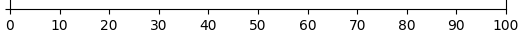
\includegraphics[scale=0.7]{images/numbers.png}
        \label{fig:tall}
    \end{figure}  
\end{frame}

\begin{frame}[fragile]{Binærsøk}
    \begin{columns}
        \begin{column}{0.50\textwidth}
            \begin{python}
def binary_search(list, target):
    left = 0
    right = len(list) - 1
    while left <= right:
        mid = (left + right) // 2
        if list[mid] == target: 
            return mid
        elif list[mid] < target: 
            left = mid + 1
        else: 
            right = mid - 1
    return -1
            \end{python}  
        \end{column}
        \begin{column}{0.47\textwidth}
            Hvor mange operasjoner blir det?\\\pause
            Vi må finne ut hvor mange ganger løkken looper.\\\pause
            I hver iterasjon blir avstanden mellom $left$ og $right$ halvert, og det kan gjøres $log_2(n)$ ganger før vi kommer til 0 eller 1.\\[2mm]\pause
            Dermed kjører et binærsøk i $log_2(n)$, som er veldig mye bedre enn $O(n)$.
        \end{column}
    \end{columns}
\end{frame}